\documentclass[border=10pt]{standalone}
\usepackage[svgnames]{xcolor}
\usepackage{amsmath}
\usepackage{pgfplots}
\pgfplotsset{compat=newest}
\usepackage[sfdefault]{FiraSans}
\usepackage{FiraMono}
\renewcommand*\familydefault{\sfdefault}
\begin{document}
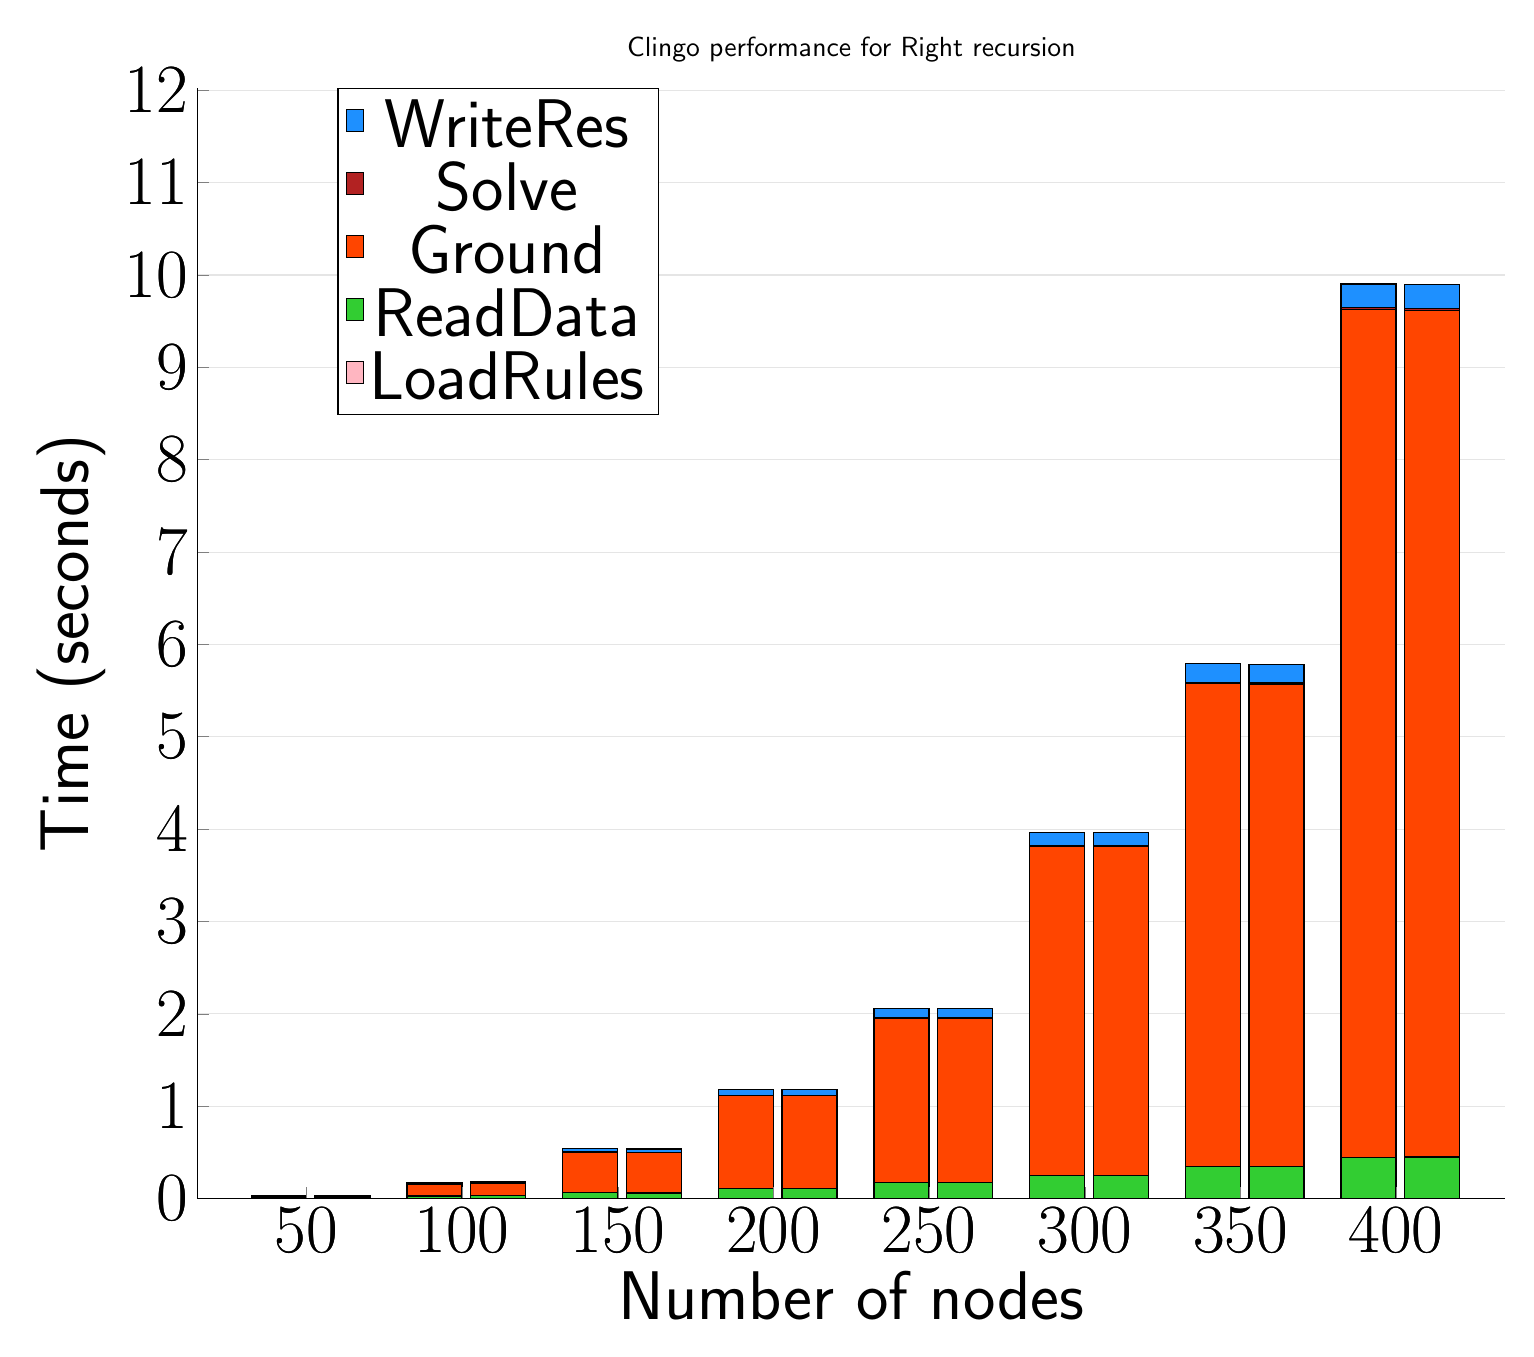
\begin{tikzpicture}
\begin{axis}[
   ybar stacked,
   title={Clingo performance for Right recursion},
   bar shift=-10pt,
   width=1.5\textwidth,
   bar width=0.7cm,
   ymajorgrids, tick align=inside,
   major grid style={draw=gray!20},
   xtick=data,
   ymin=0, ymax=12.025999999046325,
   axis x line*=bottom,
   axis y line*=left,
   enlarge x limits=0.1,
   legend style={
       at={(0.23, 1)},
       anchor=north,
       legend columns=1,
       font=\Huge,
   },
   ylabel={Time (seconds)},
   xlabel={Number of nodes},
   label style={font=\Huge},
   tick label style={font=\Huge},
]
\addlegendimage{fill=DodgerBlue, draw=black, line width=0.2pt}
\addlegendentry{WriteRes}
\addlegendimage{fill=FireBrick, draw=black, line width=0.2pt}
\addlegendentry{Solve}
\addlegendimage{fill=OrangeRed, draw=black, line width=0.2pt}
\addlegendentry{Ground}
\addlegendimage{fill=LimeGreen, draw=black, line width=0.2pt}
\addlegendentry{ReadData}
\addlegendimage{fill=LightPink, draw=black, line width=0.2pt}
\addlegendentry{LoadRules}
\addplot +[fill=LightPink, draw=black, line width=0.5pt] coordinates {
    (50, 0.0)
    (100, 0.0)
    (150, 0.0009999990463256836)
    (200, 0.0)
    (250, 0.0)
    (300, 0.0009999990463256836)
    (350, 0.0)
    (400, 0.0009999990463256836)
};
\addplot +[fill=LimeGreen, draw=black, line width=0.5pt] coordinates {
    (50, 0.006999993324279785)
    (100, 0.02799999713897705)
    (150, 0.0619999885559082)
    (200, 0.11100010871887207)
    (250, 0.17500002384185792)
    (300, 0.2509999990463257)
    (350, 0.3440000057220459)
    (400, 0.4460000038146973)
};
\addplot +[fill=OrangeRed, draw=black, line width=0.5pt] coordinates {
    (50, 0.01700000762939453)
    (100, 0.13100001811981202)
    (150, 0.43899998664855955)
    (200, 1.0039999723434447)
    (250, 1.7789999723434449)
    (300, 3.562000036239624)
    (350, 5.234999966621399)
    (400, 9.181999993324279)
};
\addplot +[fill=FireBrick, draw=black, line width=0.5pt] coordinates {
    (50, 0.0)
    (100, 0.0009999990463256836)
    (150, 0.0009999990463256836)
    (200, 0.0019999980926513673)
    (250, 0.006999993324279785)
    (300, 0.007999992370605469)
    (350, 0.01099998950958252)
    (400, 0.015999984741210938)
};
\addplot +[fill=DodgerBlue, draw=black, line width=0.5pt] coordinates {
    (50, 0.006999993324279785)
    (100, 0.01700000762939453)
    (150, 0.036999988555908206)
    (200, 0.06599996089935303)
    (250, 0.09800002574920655)
    (300, 0.1440000057220459)
    (350, 0.20100004673004152)
    (400, 0.2560000419616699)
};
\end{axis}
\begin{axis}[
   ybar stacked,
   bar shift=13pt,
   width=1.5\textwidth,
   bar width=0.7cm,
   ymajorgrids, tick align=inside,
   major grid style={draw=none},
   xtick=data,
   ymin=0, ymax=12.025999999046325,
   axis x line*=none,
   axis y line*=none,
   enlarge x limits=0.1,
   label style={font=\Huge},
   tick label style={font=\Huge},
]
\addplot +[fill=LightPink, draw=black, line width=0.5pt] coordinates {
    (50, 0.0)
    (100, 0.0)
    (150, 0.0)
    (200, 0.0)
    (250, 0.0)
    (300, 0.0)
    (350, 0.0)
    (400, 0.0)
};
\addplot +[fill=LimeGreen, draw=black, line width=0.5pt] coordinates {
    (50, 0.009999999999999997)
    (100, 0.030000000000000006)
    (150, 0.06000000000000001)
    (200, 0.11200000000000002)
    (250, 0.173)
    (300, 0.252)
    (350, 0.34700000000000003)
    (400, 0.4490000000000001)
};
\addplot +[fill=OrangeRed, draw=black, line width=0.5pt] coordinates {
    (50, 0.018000000000000006)
    (100, 0.12999999999999998)
    (150, 0.43899999999999995)
    (200, 1.001)
    (250, 1.7810000000000001)
    (300, 3.562)
    (350, 5.225)
    (400, 9.169)
};
\addplot +[fill=FireBrick, draw=black, line width=0.5pt] coordinates {
    (50, 0.0020000000000000005)
    (100, 0.0)
    (150, 0.0010000000000000009)
    (200, 0.0050000000000000044)
    (250, 0.007000000000000029)
    (300, 0.008000000000000009)
    (350, 0.011999999999999744)
    (400, 0.01700000000000017)
};
\addplot +[fill=DodgerBlue, draw=black, line width=0.5pt] coordinates {
    (50, 0.0020000000000000005)
    (100, 0.020000000000000018)
    (150, 0.036999999999999963)
    (200, 0.05999999999999996)
    (250, 0.09900000000000012)
    (300, 0.14300000000000002)
    (350, 0.1960000000000004)
    (400, 0.25899999999999945)
};
\end{axis}
\end{tikzpicture}

\end{document}
